\section{SpMV Datasets}


\begin{table}[htbp]
  \centering
  \scriptsize
  \caption{SpMV Sample Matrices}
  \vspace{-12pt}
  \label{tab:spmv_sample_matrices}
  \begin{tabular}{|
      >{\centering\arraybackslash}m{0.2\linewidth-2\tabcolsep-1.2\arrayrulewidth}|
      >{\centering\arraybackslash}m{0.2\linewidth-2\tabcolsep-1.2\arrayrulewidth}|
      >{\centering\arraybackslash}m{0.2\linewidth-2\tabcolsep-1.2\arrayrulewidth}|
      >{\centering\arraybackslash}m{0.2\linewidth-2\tabcolsep-1.2\arrayrulewidth}|
      >{\centering\arraybackslash}m{0.2\linewidth-2\tabcolsep-1.2\arrayrulewidth}|}
      \hline
       & \textbf{HB/saylr4} & \textbf{Norris/heart3} & \textbf{large\_band} & \textbf{SNAP/as-735} \\
      \hline
      \textbf{Spy} & 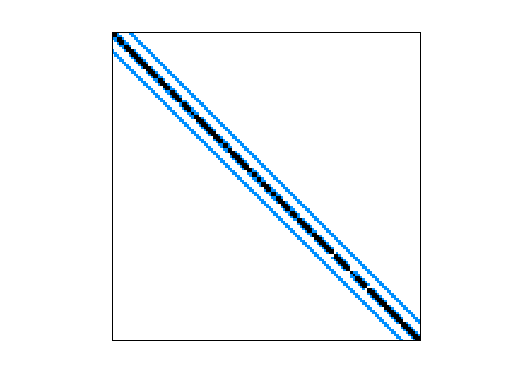
\includegraphics[width=\linewidth]{spmv_matrices/saylr4.png} & 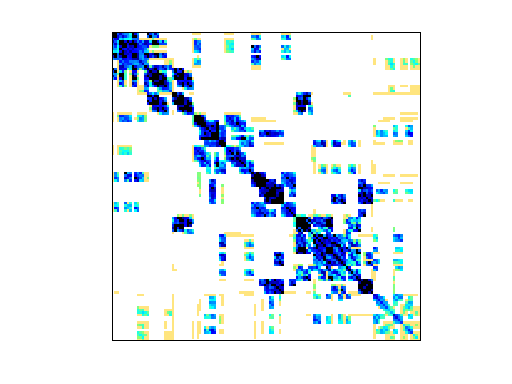
\includegraphics[width=\linewidth]{spmv_matrices/heart3.png} & 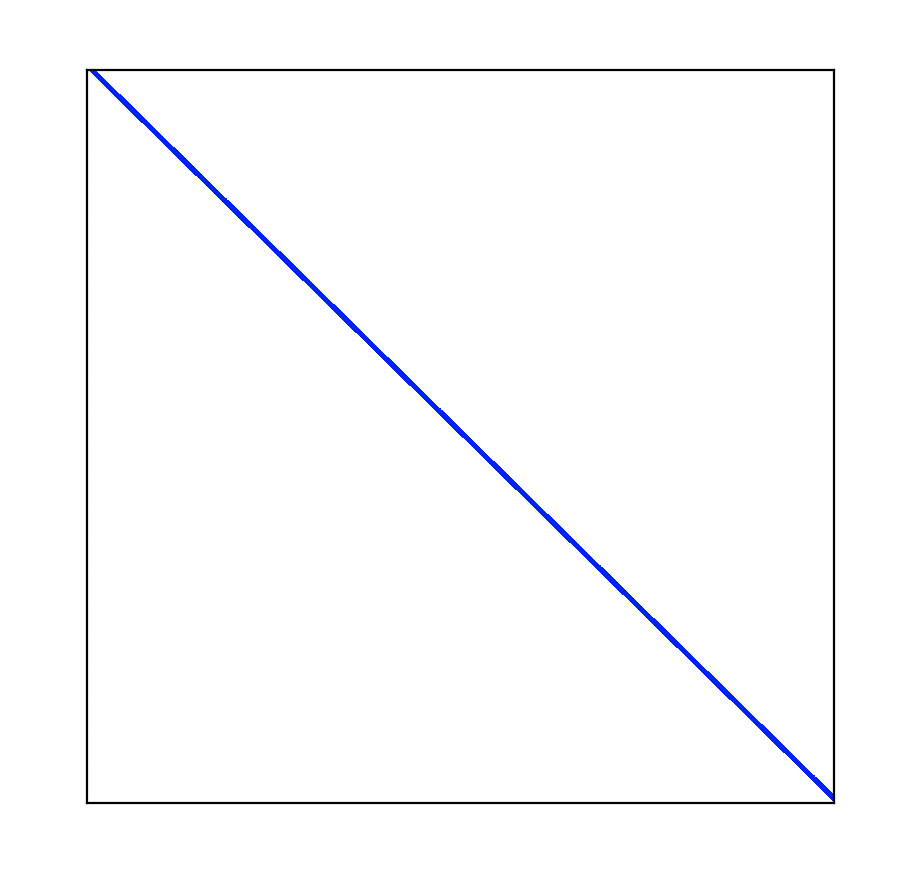
\includegraphics[width=\linewidth]{spmv_matrices/toeplitz_large_band.png} & 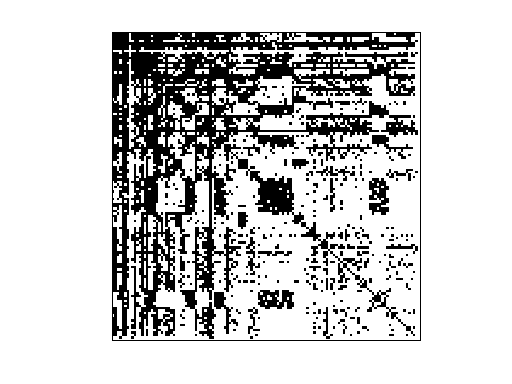
\includegraphics[width=\linewidth]{spmv_matrices/as-735.png} \\
      \hline 
      \textbf{Group / Name} & HB/saylr4 & Norris/heart3 & large\_band & SNAP/as-735 \\
      \hline
      \textbf{Dimensions} & 3,564 x 3,564 (22,316) & 2,339 x 2,339 (680,341) & 10,000 x 10,000 (1,999,900) & 7,716 x 7,716 (26,467) \\
      \hline
      \textbf{Best Finch Format} & Symmetric SparseList & SparseVBL & SparseBand & Symmetric SparseList-Pattern \\
      \hline
  \end{tabular}
  \vspace{-8pt}
\end{table}